\documentclass[conference]{IEEEtran}
\IEEEoverridecommandlockouts

\usepackage{cite}
\usepackage{amsmath,amssymb,amsfonts}
\usepackage{graphicx}
\usepackage{textcomp}
\usepackage{xcolor}
\usepackage{booktabs}
\usepackage[hidelinks]{hyperref}

\def\BibTeX{{\rm B\kern-.05em{\sc i\kern-.025em b}\kern-.08em
    T\kern-.1667em\lower.7ex\hbox{E}\kern-.125emX}}

\begin{document}

\title{DeepLabV3 with Pretrained Backbone for Semantic Segmentation on Cityscapes}

\author{\IEEEauthorblockN{Jochem Plegt}
\IEEEauthorblockA{\textit{Eindhoven University of Technology}}}

\maketitle

\begin{abstract}
Semantic segmentation in autonomous driving requires models that are both accurate and robust to real-world image corruptions. This paper proposes replacing the baseline U-Net with a DeepLabV3 model using a pretrained ResNet-50 backbone, combined with data augmentation (random horizontal flipping and color jitter) and cosine annealing learning rate scheduling. To preserve the pretrained BatchNorm statistics, the backbone is frozen during training. Experiments on the Cityscapes dataset show a modest improvement in peak performance (Mean Dice 0.4681 vs.\ 0.4598) and a substantially larger improvement in robustness under common image corruptions (Mean Dice 0.4108 vs.\ 0.2079), retaining 87.8\% of clean performance compared to only 45.2\% for the baseline. These results demonstrate that pretrained backbones and data augmentation are highly effective for building robust semantic segmentation models.
\end{abstract}

\begin{IEEEkeywords}
Semantic Segmentation, DeepLabV3, Pretrained Backbone, Data Augmentation, Robustness
\end{IEEEkeywords}


%% -------------------------------------------------------
\section{Introduction}

Semantic segmentation is a fundamental task in computer vision, where the goal is to assign a class label to every pixel in an image. In safety-critical applications such as autonomous driving, accurate segmentation is essential — misclassifications can have life-threatening consequences \cite{grigorescu2020survey}.

However, deploying segmentation models in the real world is challenging. Images captured by autonomous vehicles are subject to varying lighting conditions, weather effects, and sensor noise. Models trained from scratch on a fixed dataset may fail to generalize under such conditions, producing incorrect predictions that are difficult to anticipate.

The baseline approach for this task is a U-Net architecture \cite{ronneberger2015unet}, which uses an encoder-decoder structure with skip connections to combine high-level semantic features with low-level spatial information. While effective, U-Net is trained from scratch and therefore relies entirely on the training data distribution. This makes it potentially vulnerable to variations in image quality that were not present during training.

DeepLabV3 \cite{chen2017deeplab} offers a more powerful alternative, using dilated convolutions and atrous spatial pyramid pooling (ASPP) to capture multi-scale context without reducing resolution. When paired with a ResNet-50 backbone \cite{he2016resnet} pretrained on ImageNet \cite{russakovsky2015imagenet}, the model benefits from rich feature representations learned on millions of images. While pretrained backbones are known to improve segmentation performance, their effect on robustness under real-world image corruptions remains underexplored.

This motivates the research question: \textit{does replacing the baseline U-Net with a DeepLabV3 model using a pretrained ResNet50 backbone, combined with data augmentation, improve both segmentation performance and robustness to image corruptions on the Cityscapes dataset?}

To answer this, a DeepLabV3-ResNet50 model is trained on Cityscapes \cite{cordts2016cityscapes} and evaluated on both the peak performance and robustness benchmarks, and compared against the baseline U-Net.

The code used to produce the results presented in this paper is publicly available at: \url{https://github.com/JochemPlegt/5LSM0_NN_jochem}.


%% -------------------------------------------------------
\section{Related Work}

\subsection{Semantic Segmentation}
Various architectures have been proposed for semantic segmentation. U-Net \cite{ronneberger2015unet} follows an encoder-decoder structure with skip connections, which allow high-level semantic features to be combined with low-level spatial features to better capture fine details. Originally designed for biomedical image segmentation, U-Net has proven effective across many segmentation tasks due to its simple structure and efficient training from scratch. DeepLabV3 \cite{chen2017deeplab} uses dilated convolutions and atrous spatial pyramid pooling (ASPP) to capture features at multiple scales without reducing spatial resolution, making it particularly suited for datasets with complex urban scenes such as Cityscapes \cite{cordts2016cityscapes}. The Cityscapes dataset contains 5000 finely annotated urban street scene images across 19 semantic classes, and serves as a standard benchmark for semantic segmentation.

\subsection{Pretrained Backbones}
DeepLabV3 can be paired with a ResNet-50 backbone \cite{he2016resnet} pretrained on ImageNet \cite{russakovsky2015imagenet}. ResNet-50 contains approximately 25 million parameters and uses residual connections to enable training of deep networks without vanishing gradients. Pretraining on the ImageNet dataset — which contains over 1.2 million images across 1000 classes — allows the backbone to learn general-purpose feature representations, which transfer well to downstream tasks such as semantic segmentation. However, when fine-tuning a pretrained backbone on a new dataset, the BatchNorm running statistics accumulated during pretraining can be corrupted by updates on the smaller target dataset, leading to a discrepancy between training and evaluation performance. Freezing the backbone during fine-tuning preserves these statistics and stabilizes training.

\subsection{Robustness}
Hendrycks and Dietterich \cite{hendrycks2019robustness} introduced a benchmark for evaluating the robustness of neural networks to common image corruptions, such as noise, blur, and weather effects. Their work shows that standard models trained on clean data suffer significant performance degradation under such corruptions, which is particularly problematic for safety-critical applications like autonomous driving \cite{grigorescu2020survey}. Data augmentation during training, such as color jitter and random flipping, has been shown to improve robustness by exposing the model to a wider variety of inputs during training.


%% -------------------------------------------------------
\section{Methodology}

\subsection{Datasets and Preprocessing}
The Cityscapes dataset \cite{cordts2016cityscapes} is used as the training and validation set, containing urban street scenes annotated with 19 semantic classes. The original training and validation splits are used. All images are resized to $256 \times 256$ pixels and normalized using ImageNet channel-wise mean $(0.485, 0.456, 0.406)$ and standard deviation $(0.229, 0.224, 0.225)$.

During training, two data augmentation techniques are applied: random horizontal flipping, applied jointly to the image and its label mask, and color jitter (brightness, contrast, saturation, and hue), applied to the image only before normalization. These augmentations are applied only during training to improve generalization.

\subsection{Model Architecture}
Two models are evaluated: a baseline U-Net and a DeepLabV3-ResNet50 model. The U-Net follows a standard encoder-decoder structure with four downsampling and four upsampling blocks using double convolutions. The DeepLabV3 model uses a ResNet-50 backbone pretrained on ImageNet, with the classifier head replaced by a $1 \times 1$ convolution producing 19 output channels for the Cityscapes classes. The auxiliary classifier is removed. All models are implemented in PyTorch.

To prevent corruption of the pretrained BatchNorm statistics during fine-tuning, the backbone parameters are frozen and its BatchNorm layers are kept in evaluation mode throughout training. Only the classifier head is trained from scratch.

\subsection{Training}
Both models are trained on the Cityscapes training split for 100 epochs using the AdamW optimizer and cross-entropy loss with ignore index 255 for void pixels, with a batch size of 64. The baseline U-Net is trained with a fixed learning rate of 0.001. The DeepLabV3-ResNet50 model is trained with a learning rate of 0.001 and cosine annealing scheduling, which gradually reduces the learning rate to zero over the course of training.

The baseline U-Net achieved its best validation loss at epoch 46. The DeepLabV3-ResNet50 model reached its best validation loss of 0.3585 at epoch 31, after which slight overfitting was observed. The checkpoint from this optimal epoch was saved for evaluation. Fig.~\ref{fig:loss} shows the training and validation loss curves for the DeepLabV3-ResNet50 model.

\begin{figure}[h]
    \centering
    \begin{minipage}{0.48\linewidth}
        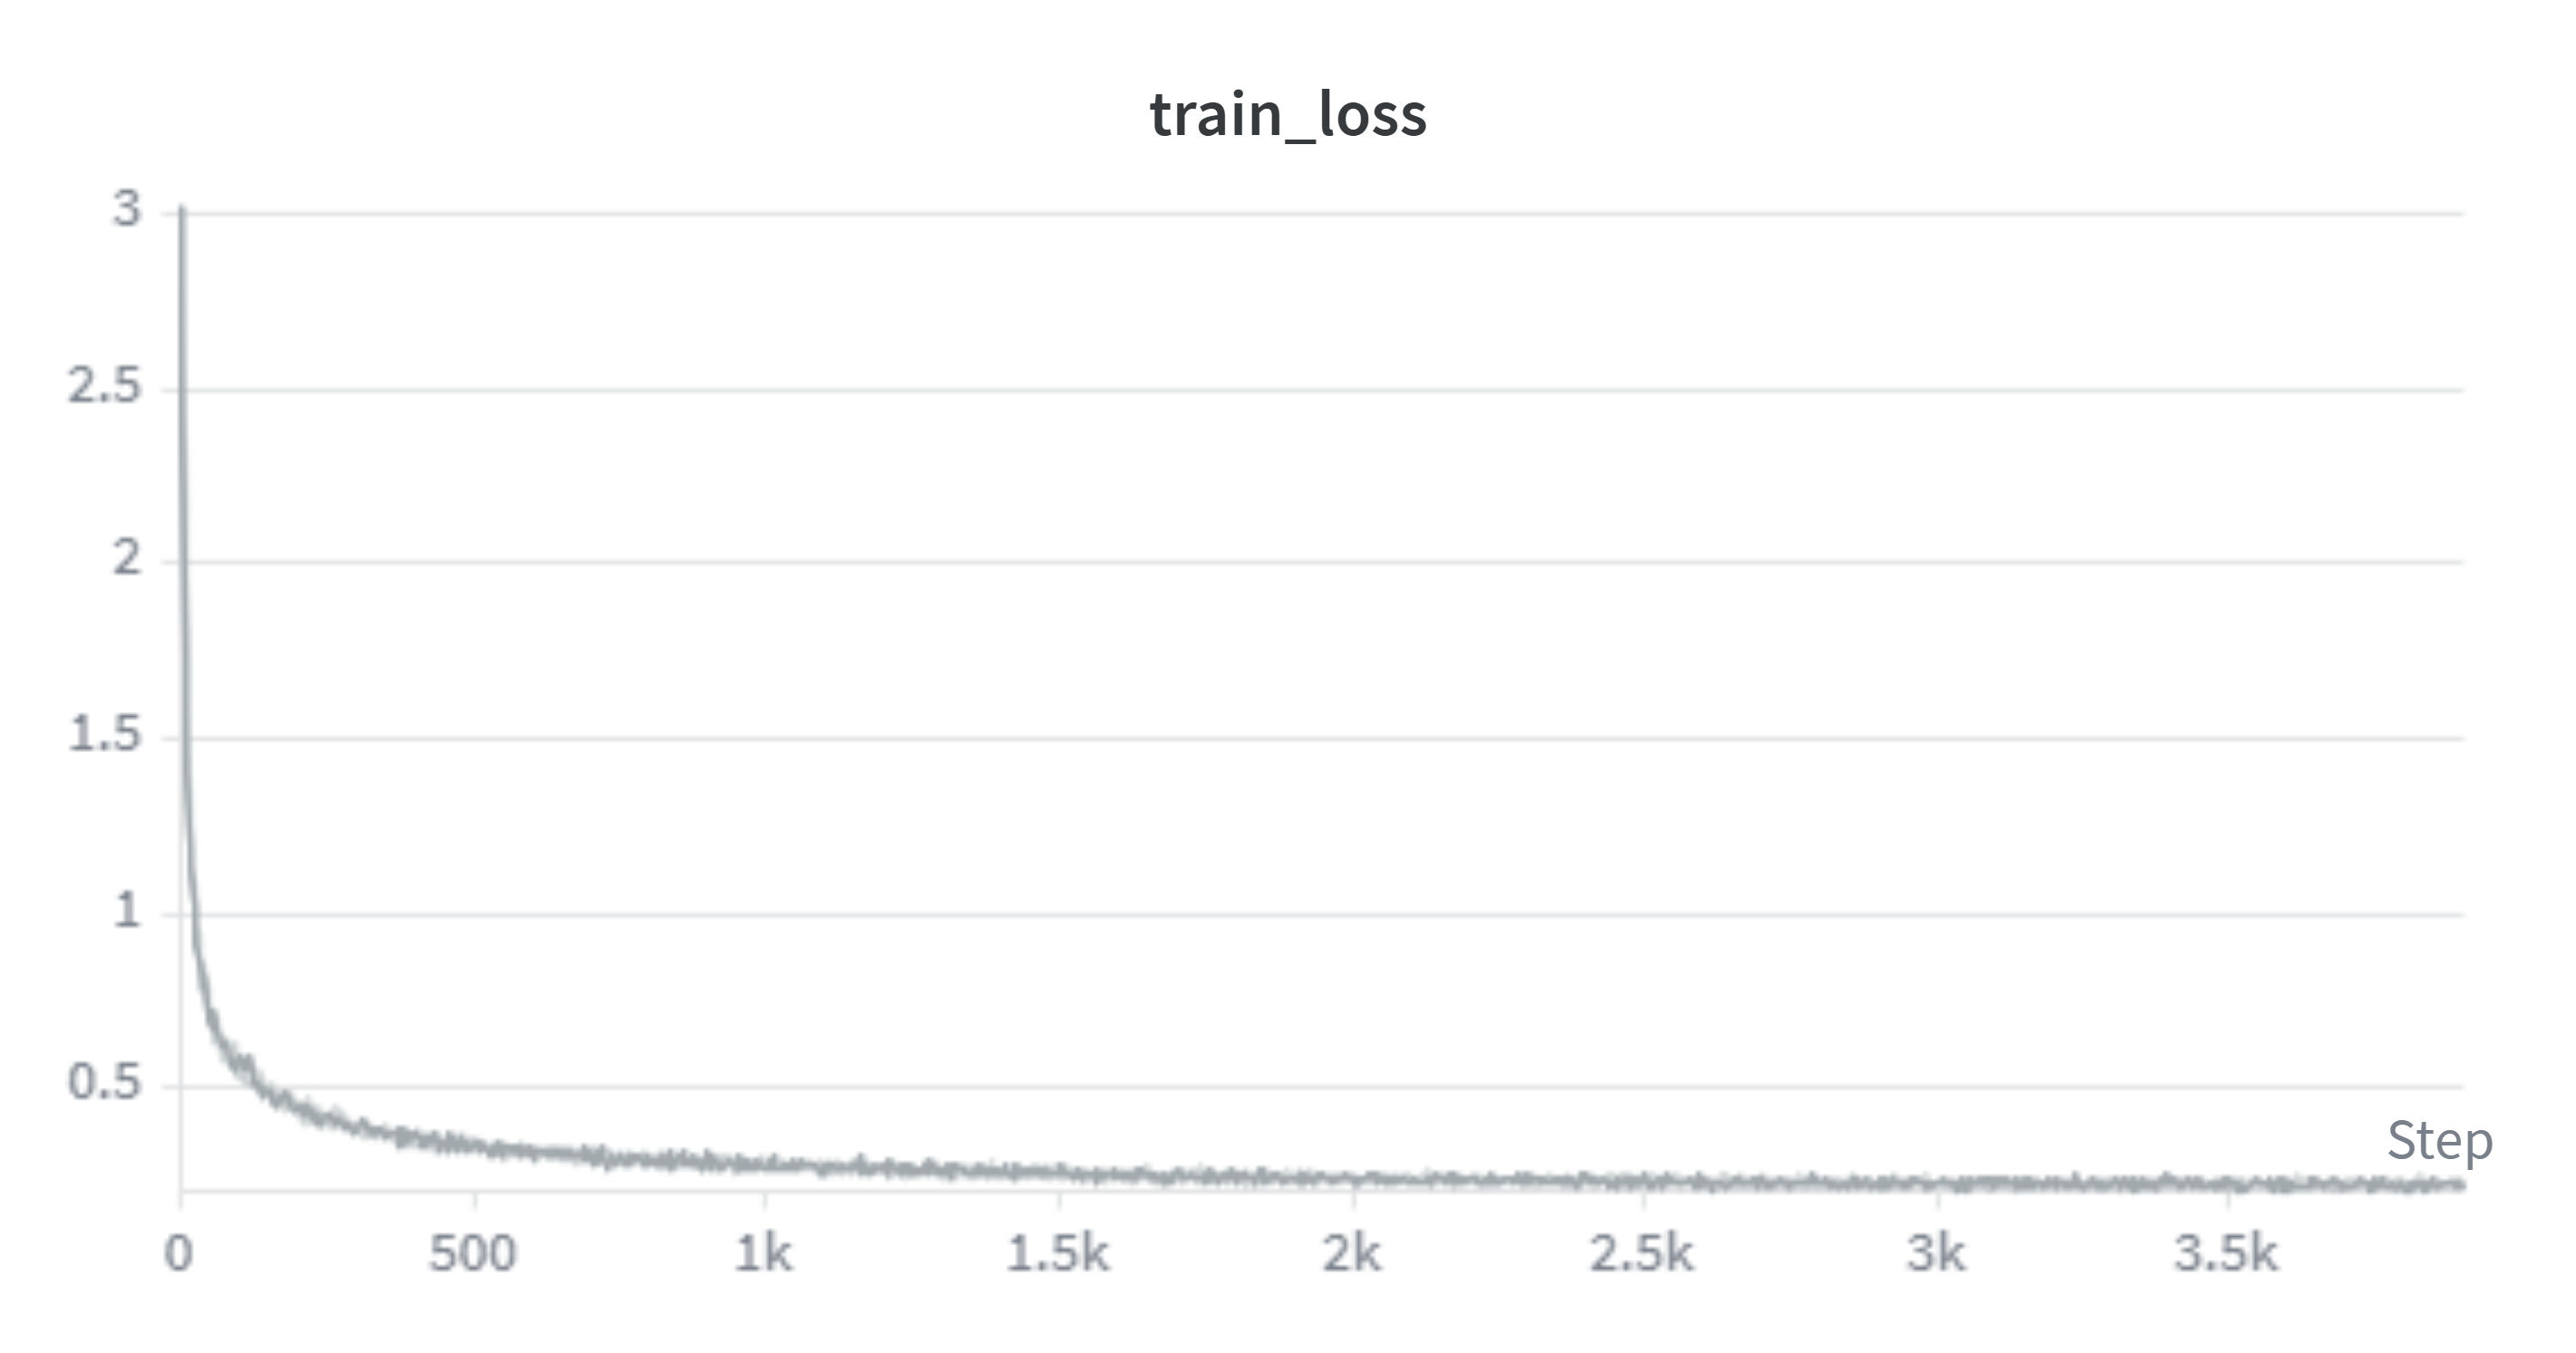
\includegraphics[width=\linewidth, height=3cm, keepaspectratio]{figures/deeplabv3_train_loss.png}
    \end{minipage}
    \hfill
    \begin{minipage}{0.48\linewidth}
        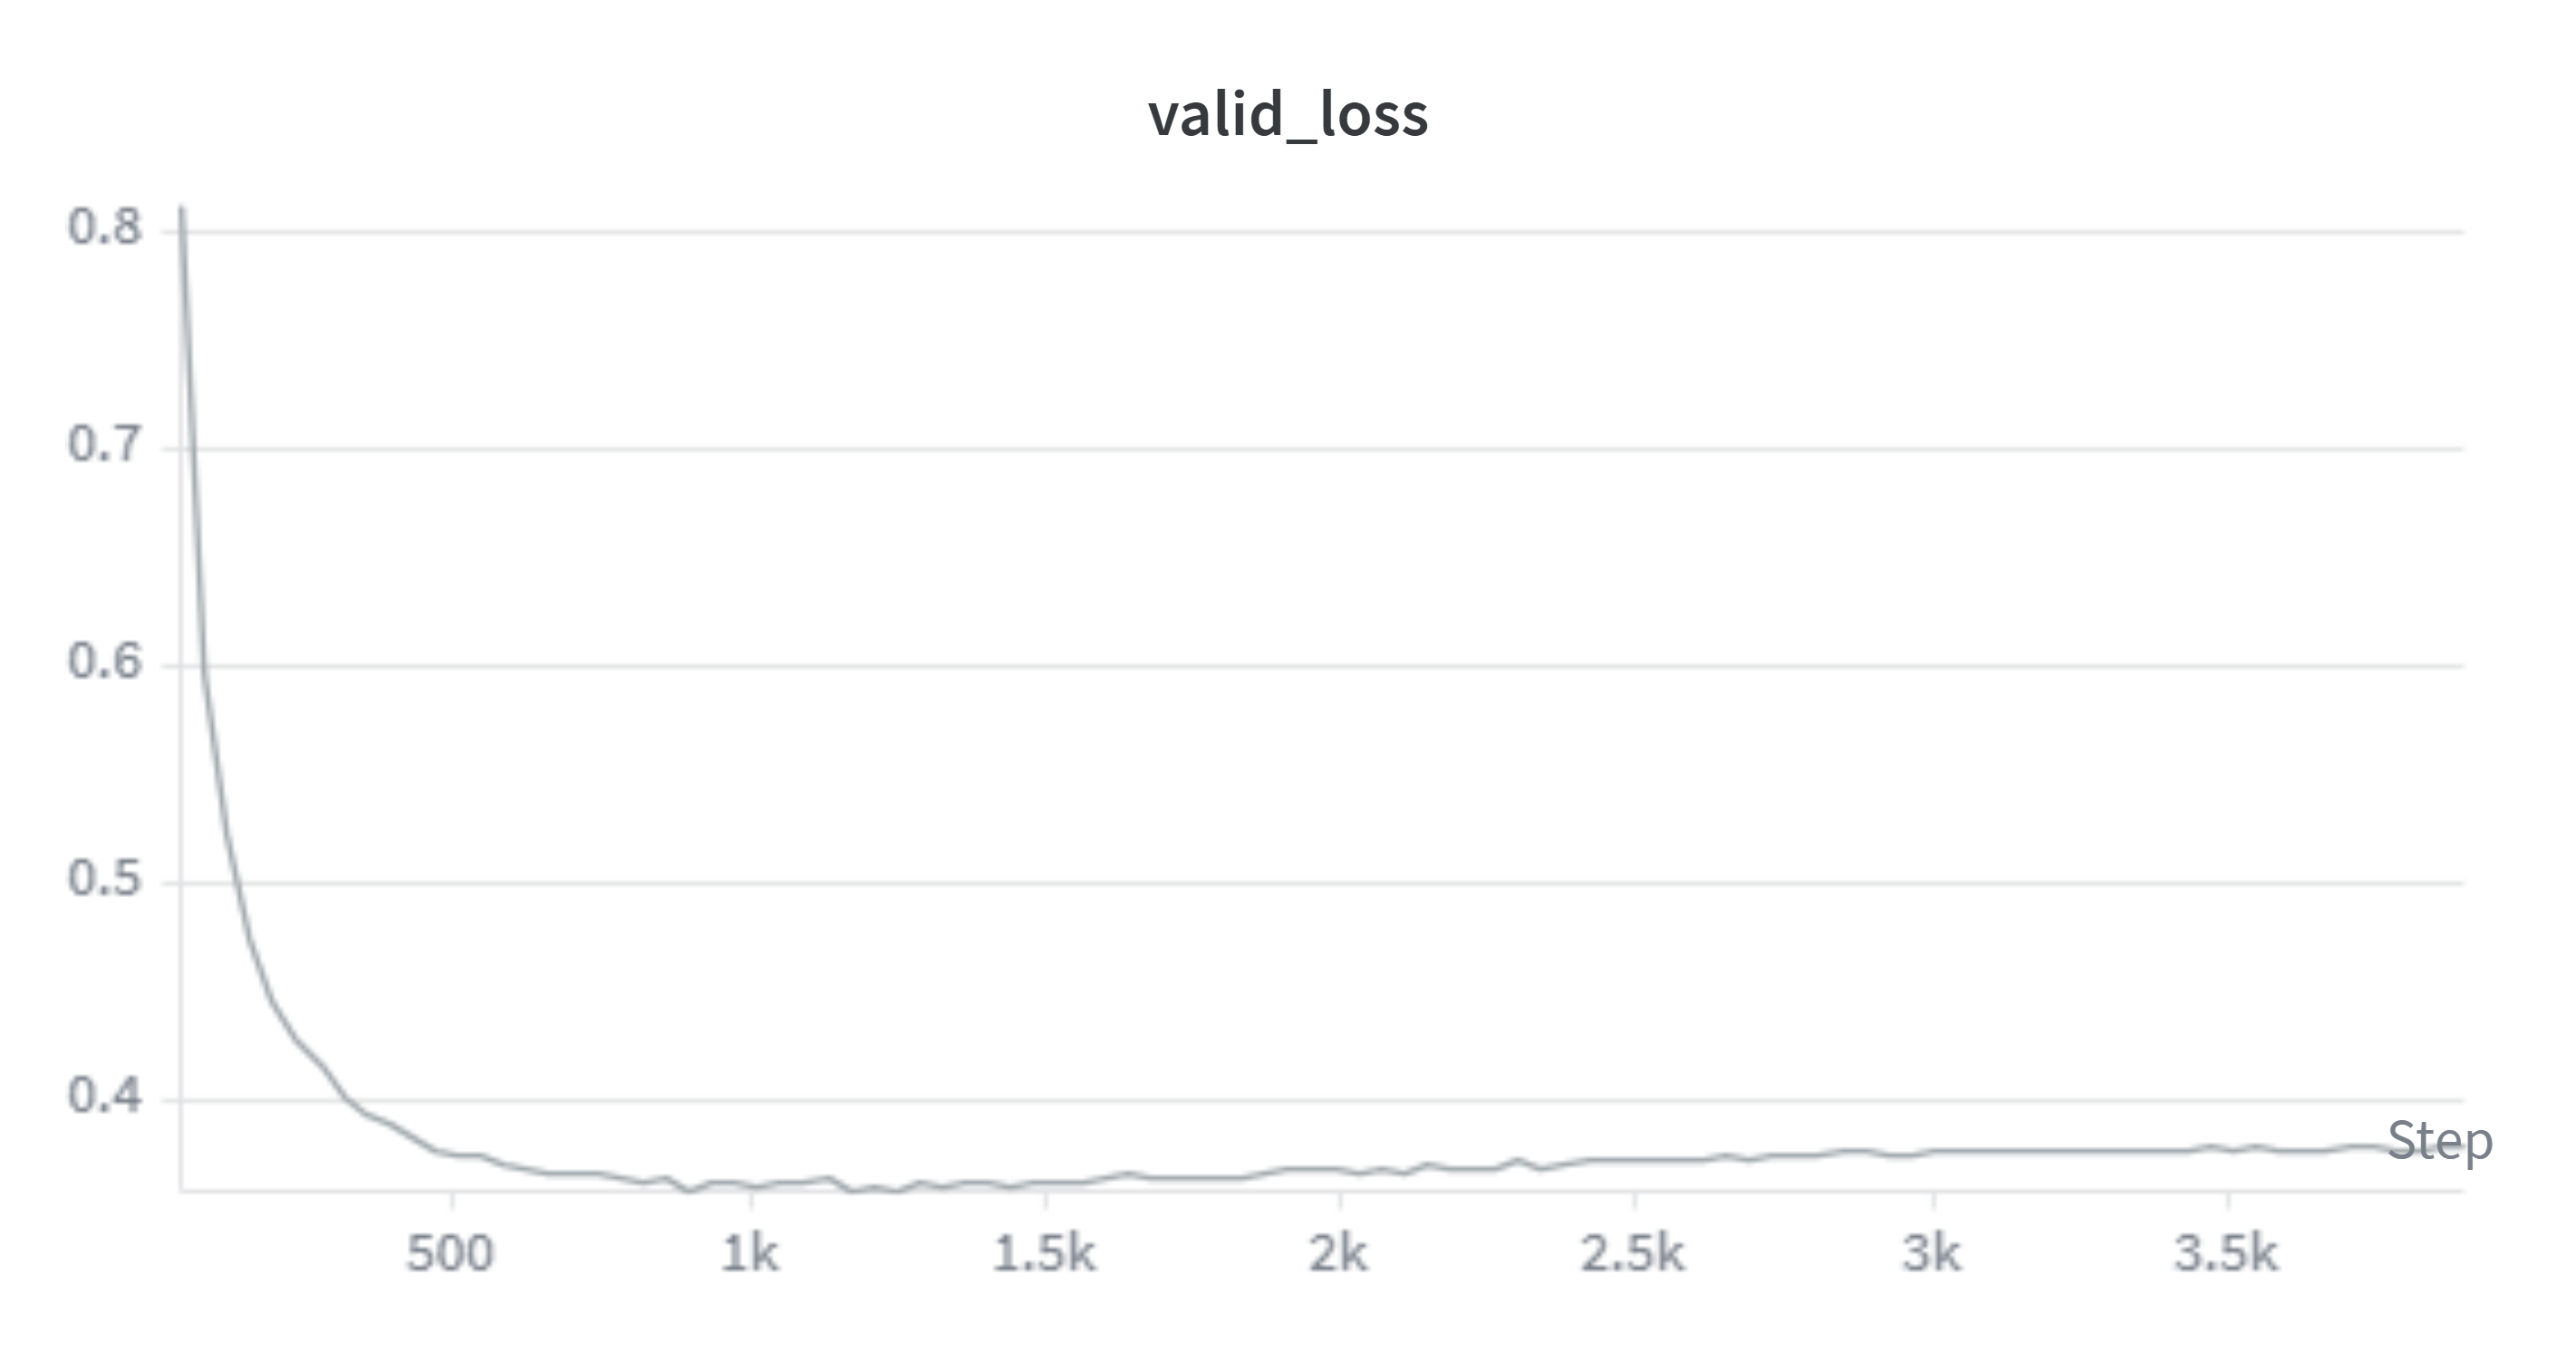
\includegraphics[width=\linewidth, height=3cm, keepaspectratio]{figures/deeplabv3_valid_loss.png}
    \end{minipage}
    \caption{Training loss (left) and validation loss (right) of the DeepLabV3-ResNet50 model over 100 epochs. The validation loss reaches its minimum around epoch 31, after which slight overfitting is observed.}
    \label{fig:loss}
\end{figure}

\subsection{Evaluation}
Model performance is evaluated on two benchmarks. For \textit{peak performance}, the Mean Dice score and Mean IoU are measured on the clean Cityscapes test set. For \textit{robustness}, the same metrics are measured on a corrupted version of the test set, containing common image corruptions such as noise, blur, and weather effects \cite{hendrycks2019robustness}. Both benchmarks are evaluated through the challenge submission server.


%% -------------------------------------------------------
\section{Results}

\subsection{Peak Performance}

Table~\ref{tab:peak} reports the peak performance results on the clean Cityscapes test set. The DeepLabV3-ResNet50 model achieves a Mean Dice score of 0.4681 and a Mean IoU of 0.3887, compared to 0.4598 Mean Dice and 0.3758 Mean IoU for the baseline U-Net. While the improvement in peak performance is modest, the DeepLabV3 model consistently outperforms the baseline across most semantic categories.

\begin{table}[h]
\centering
\caption{Peak performance on the clean Cityscapes test set.}
\label{tab:peak}
\begin{tabular}{lcc}
\toprule
Model & Mean Dice & Mean IoU \\
\midrule
Baseline U-Net & 0.4598 & 0.3758 \\
DeepLabV3-ResNet50 & 0.4681 & 0.3887 \\
\bottomrule
\end{tabular}
\end{table}

\subsection{Robustness}

Table~\ref{tab:robustness} reports the robustness results on the corrupted Cityscapes test set. The DeepLabV3-ResNet50 model achieves a Mean Dice score of 0.4108 and a Mean IoU of 0.3358 under corruptions, compared to only 0.2079 Mean Dice for the baseline U-Net. This represents a relative improvement of approximately 98\% in Mean Dice, demonstrating substantially better robustness.

\begin{table}[h]
\centering
\caption{Robustness results on the corrupted Cityscapes test set.}
\label{tab:robustness}
\begin{tabular}{lcc}
\toprule
Model & Mean Dice & Mean IoU \\
\midrule
Baseline U-Net & 0.2079 & 0.1539 \\
DeepLabV3-ResNet50 & 0.4108 & 0.3358 \\
\bottomrule
\end{tabular}
\end{table}

Fig.~\ref{fig:predictions} shows example segmentation predictions produced by the DeepLabV3-ResNet50 model on the Cityscapes validation set. The model produces spatially coherent segmentation maps with clear boundaries between semantic categories such as road, vegetation, and buildings.

\begin{figure}[h]
    \centering
    \begin{minipage}{0.48\linewidth}
        
\includegraphics[width=\linewidth]{figures/deeplabv3_pred1.png}
    \end{minipage}
    \hfill
    \begin{minipage}{0.48\linewidth}
        
\includegraphics[width=\linewidth]{figures/deeplabv3_pred2.png}
    \end{minipage}
    \caption{Example segmentation predictions by the DeepLabV3-ResNet50 model on the Cityscapes validation set. Colors correspond to semantic classes (e.g., purple: road, green: vegetation, blue: vehicle).}
    \label{fig:predictions}
\end{figure}

Fig.~\ref{fig:per_category} shows the per-category Dice scores under corruptions. The DeepLabV3 model outperforms the baseline across all semantic categories, with particularly large improvements in the Flat (road, sidewalk) and Construction (building, wall, fence) categories.

\begin{figure}[h]
    \centering
    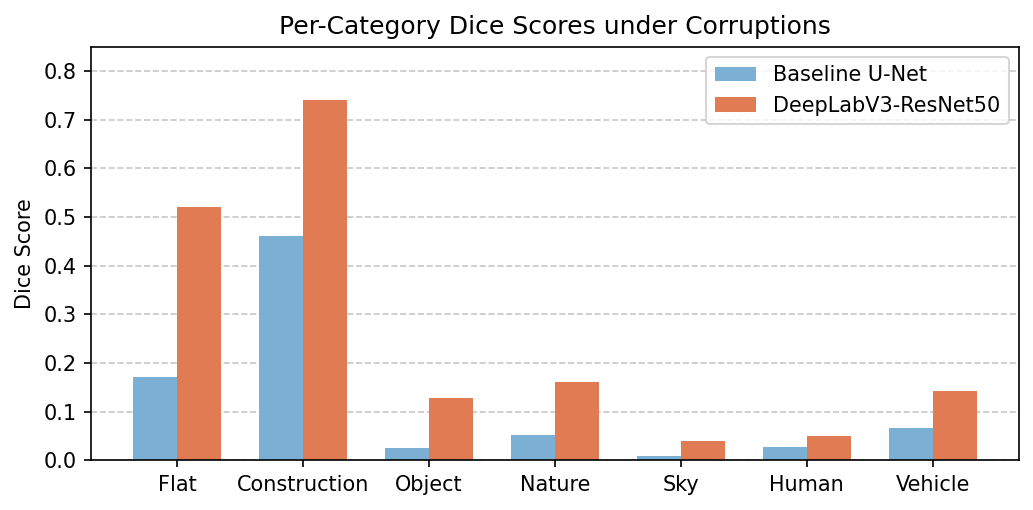
\includegraphics[width=\linewidth]{figures/robustness_per_category.png}
    \caption{Per-category Dice scores on the corrupted test set for the baseline U-Net and DeepLabV3-ResNet50.}
    \label{fig:per_category}
\end{figure}

The large gap in robustness can be attributed to two factors. First, the pretrained ResNet-50 backbone provides feature representations learned on millions of diverse ImageNet images, making the model less sensitive to the specific appearance of clean Cityscapes images. Second, data augmentation during training — in particular color jitter — exposes the model to a wider range of visual conditions, improving generalization under corruptions.

The per-category breakdown reveals that the largest absolute improvements occur in the Flat (+0.349) and Construction (+0.278) categories. These large-area categories, which dominate the urban scene, benefit most from the richer spatial representations provided by the ASPP module and pretrained backbone. Smaller categories such as Human and Object show more modest gains, likely due to the limited number of training examples and the difficulty of segmenting small objects under image corruptions.

Notably, the DeepLabV3 model retains 87.8\% of its clean performance under corruptions (0.4108 / 0.4681), while the baseline U-Net retains only 45.2\% (0.2079 / 0.4598). This confirms that the proposed approach significantly improves robustness beyond what would be expected from the modest peak performance gain alone.


%% -------------------------------------------------------
\section{Conclusion and Discussion}

This paper investigated whether replacing the baseline U-Net with a DeepLabV3 model using a pretrained ResNet-50 backbone, combined with data augmentation and cosine annealing scheduling, improves both segmentation performance and robustness on the Cityscapes dataset.

The results show that DeepLabV3-ResNet50 achieves a modest improvement in peak performance (Mean Dice 0.4681 vs.\ 0.4598). The improvement is modest because the classifier head is trained from scratch on only 2975 training images, which limits the model's ability to fully exploit the pretrained backbone. The backbone itself is frozen and therefore does not adapt to Cityscapes-specific features, which may prevent further peak performance gains.

The improvement in robustness is substantially larger (Mean Dice 0.4108 vs.\ 0.2079 under corruptions). The DeepLabV3 model retains 87.8\% of its clean performance under corruptions, compared to only 45.2\% for the baseline U-Net. This large gap suggests that pretrained ImageNet features are inherently more robust to low-level image corruptions, since they were learned from a much more diverse set of images. The color jitter augmentation further contributes to this robustness by simulating appearance variations during training.

The per-category analysis reveals that smaller object categories such as Human and Object show limited improvement. This is likely due to the small pixel area these categories occupy in each image, making them harder to segment correctly under corruptions regardless of the model architecture.

Limitations of this work include the fully frozen backbone, which prevents adaptation to the Cityscapes domain. Additionally, all images are resized to $256 \times 256$ pixels, which may reduce fine-grained detail for small objects. Future work could explore gradually unfreezing backbone layers, using higher input resolutions, or applying stronger augmentation techniques such as CutMix or RandAugment to further improve both peak performance and robustness.


%% -------------------------------------------------------
\bibliographystyle{IEEEtran}
\bibliography{references}

\end{document}
